\begin{figure}[H]
  \centering
  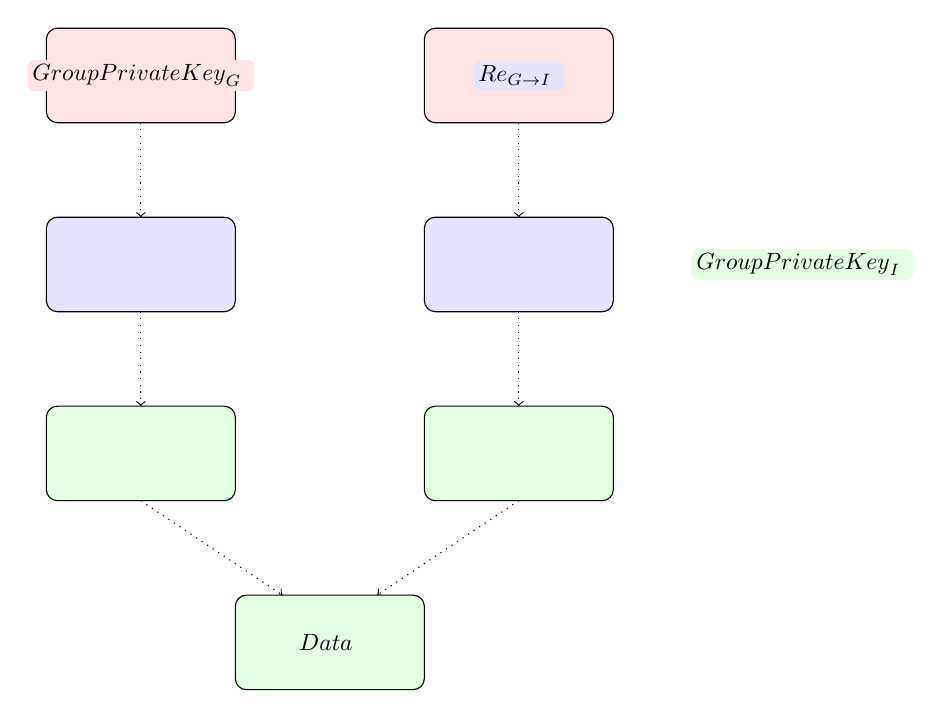
\begin{tikzpicture}[scale = 0.6, every node/.style={scale = 0.85}, every node/.append style={fill = white, rounded corners = 2pt, inner sep = 2pt, align = center}]

  % ------------------------------------------------------------------------

  \draw [rounded corners, fill=red!10] (-6, 1) rectangle (-10, -1);
  \node [fill=red!10] at (-8, 0) { $\text{Data}_{\text{SCO}}$ };

  \draw [ -> , dotted] (-8, -1) -- (-8, -3);

  \draw [rounded corners, fill=blue!10] (-6, -3) rectangle (-10, -5);
  \node [fill=blue!10] at (0, 0) { $\text{Re}_{\text{SCO} \rightarrow \text{G}}$ };

  \draw [ -> , dotted] (-8, -5) -- (-8, -7);

  \draw [rounded corners, fill=green!10] (-6, -7) rectangle (-10, -9);
  \node [fill=green!10] at (6, -4) { $\text{Data}_{\text{G}}$ };

  % ------------------------------------------------------------------------

  \draw [rounded corners, fill=red!10] (-2, 1) rectangle (2, -1);
  \node [fill=red!10] at (-8, 0) { $\text{Group Private Key}_{\text{G}}$ };

  \draw [ -> , dotted] (0, -1) -- (0, -3);

  \draw [rounded corners, fill=blue!10] (-2, -3) rectangle (2, -5);
  \node [fill=blue!10] at (0, 0) { $\text{Re}_{\text{G} \rightarrow \text{I}}$ };

  \draw [ -> , dotted] (0, -5) -- (0, -7);

  \draw [rounded corners, fill=green!10] (-2, -7) rectangle (2, -9);
  \node [fill=green!10] at (6, -4) { $\text{Group Private Key}_{\text{I}}$ };

  % ------------------------------------------------------------------------

  \draw [ -> , dotted] (-8, -9) -- (-5, -11);
  \draw [ -> , dotted] (0, -9) -- (-3, -11);

  \draw [rounded corners, fill=green!10] (-6, -11) rectangle (-2, -13);
  \node [fill=green!10] at (-4, -12) { $\text{Data}$ };

  % ------------------------------------------------------------------------

  \end{tikzpicture} \\
  \caption{
  	Group Read Re-encryption (practical)
  }{
    The practical process of re-encrypting from a storage contract owner to a group, re-encrypting a group key from the group to an individual (member of the group), and combining the two to provide the decrypted data.
  }
  \label{fig:encryption_group_read_practical}
\end{figure}
